\documentclass[../thesis.tex]{subfiles}
\begin{document}
\chapter{Discussion}\label{cap:discussion}

\section{Hand gestures}
To choose the dynamic hand gestures to use I took inspiration from the literature. I tried to invent my own gestures but, without the possibility to perform a preliminary study involving people from the context of use, it would have resulted in unrealistic and unusable gestures in the real world.\\

Regarding the static hand gestures, the choice to use the \acrshort{ASL} seemed an obvious choice to me because it is the common way to express letters using hands in societies where the Latin alphabet is used.

\section{Deep learning models}
The results achieved with the deep learning models to recognize hand gestures are astonishing. The choice to use MediaPipe has proven to be a winning one. While I was designing the \acrshort{ML} part of the project, I took into consideration the idea of using a YOLO network to recognize the hand gestures because it is known as one of the best networks to work on images and videos. But, the downside of this choice would have been the necessity of a large dataset to train the network. On the Internet, there are a lot of projects that use YOLO to recognize hand gesture.\footnote{\href{https://www.kaggle.com/search?q=hand+gesture}{https://www.kaggle.com/search?q=hand+gesture}} However, none of them are easily adaptable to different scenarios, or, to put it another way, it is extremely difficult to add a new gesture. Moreover, YOLO utilizes images or sequences of them in the case of video, and this is another drawback because when training on images, the network has to manage the environment (i.e., where the image is taken), the lightning, and also the skin color.\\

The method utilized (i.e. MediaPipe's landmarks coordinates plus a simple feed-forward neural network) leaves all the above-explained drawbacks to MediaPipe engineers because it uses only the landmarks' coordinates (i.e. numbers) to classify the different hand gestures. Obviously, MediaPipe could be substituted with another \acrshort{ML} model capable of performing hand tracking and returning the coordinates of the conjunctions of the hand, but, looking at the results obtained, it seems to be a very good solution.

\subsection{Static hand gestures recognizer}
The feed-forward deep neural network used to classify the static hand gestures turned out to be a very good solution with an accuracy greater than the $99\%$ and a time of only $6$ seconds to train it. Moreover, the results show that it works even with a very small dataset. Furthermore, the time to add a new gesture and train the network is very low.

\subsection{Dynamic hand gestures recognizer}
The two kinds of networks tested, the feed forward network and the \acrshort{LSTM} network, achieved similar results. I expected that the latter would perform better than the former because the \acrshort{LSTM} network should achieve better results in the context where past data matters. A difference could not be noticed because of the short sequence of landmarks that have been used to train the networks.\\

Moreover, the results show that the more landmarks are taken into consideration, the more accurate the prediction is. When the tips of all fingers are used, the network achieves an accuracy of $98\%$. Instead, with just the tip of the index finger, the accuracy is $93\%$, and the difference increases if the dataset size is reduced. Furthermore, the time spent on training the network is doubled when the \textit{one\_finger} dataset is used.

\section{Integration with ROS}
The requirement to work with \acrshort{ROS} has been fulfilled. The implementation allows other users to expand the capabilities of the framework. Up to now, it can work with Nav2 to guide the robot to a position and send any type of message to the robot utilizing the \acrshort{ROS} topic. In the future, the framework could be expanded, making it compatible with other packages and more \acrshort{ROS}' built-ins.

\section{Resource utilization}
The data in~\ref{ss:system_resource_usage_training} shows that the training process is fast and not resource-demanding. During the training, RAM consumption is only $2\%$ of $16GB$. Meanwhile, the CPU usage is around $14\%$ in the case of the static hand gesture recognizer and $8\%$ in the case of the dynamic hand gesture recognizer.\\

The data gathered during the simulations about the system resource utilization shows that the framework is not resource demanding. All simulations were run in a virtual machine equipped with a $4$ CPU core and $8GB$ of RAM. Regarding the CPU, the results show that after the initialization (the first spike in figure~\ref{fig:cpu_usage}) the utilization is between $12\% -14\%$. While, as far as RAM is concerned, its occupancy stabilizes below $7\%$ and thus for a total of $\sim 560MB$.\\

Looking at the results, NVIDIA's Jetson Nano, with its $4GB$ of RAM, a four core CPU, and GPU, could be taken into consideration as a possible hardware to test the framework in a real environment. Maybe one of the latest Raspberry-Pi could handle it as well. This is an important fact because those two micro-computers are among the most widely used for the development of robotic applications.
 
\section{Complexity score}
There is no common way to evaluate the complexity of a JSON file, as explained in~\ref{sss:automaton_methodology}. The method adopted has been chosen to give an objective evaluation of the difficulty of writing and reading a JSON file to meet the non-functional requirement of being easily configurable.

Therefore, it is important to have a low complexity score obtained. To achieve this goal, it is important to wisely design the automaton that describes the accepted input. For example, one can verify that the represented automaton is in its minimized version. The automaton obtained from the configuration can be proven to be in its minimized version.

\section{Problems}
The solution proposed is not without issues. An easy to fix one is the lack of functionalities regarding the integration with \gls{ROS}. Up to now, the integration is just at the beginning. The framework can only work with Nav2 as the navigation system and can only send messages through topics. Thanks to how it has been implemented, the framework's developers can integrate new functionalities and other packages very easily. It is sufficient to write the wrapper and update the accepted actions in the \texttt{AutomataManager} class.

Another problem regards MediaPipe. It is a black box from the point of view of the implementation because the framework gives in input a frame and receives in output a list of landmarks. As explained in~\ref{sec:mediapipe}, MediaPipe is a very good tool with a high level of accuracy, but it is not without problems. For example, in some scenarios it can not recognize the hand, and without that functionality, the whole framework falls apart. Figure~\ref{fig:ht_with_and_without_glove} shows the difference when the users wear a glove and when they do not. In figure~\ref{fig:ht_without_gloves} the hand tracking works perfectly as the presence of landmarks is highlighted by the black dots on the hand. Meanwhile, in figure~\ref{fig:ht_with_gloves}, the glove prevents MediaPipe from working correctly and no landmark is recognized. This is an important threat to the framework's functionality as it could be used in some environments where the users wear clothes or there are other things that block the key component of the framework from doing its job. Most importantly, there is nothing that can be done to resolve this issue other than to wait for MediaPipe's engineer to find a solution or change tool.
\begin{figure}
    \centering
    \begin{subfigure}[b]{1\textwidth}
        \centering
        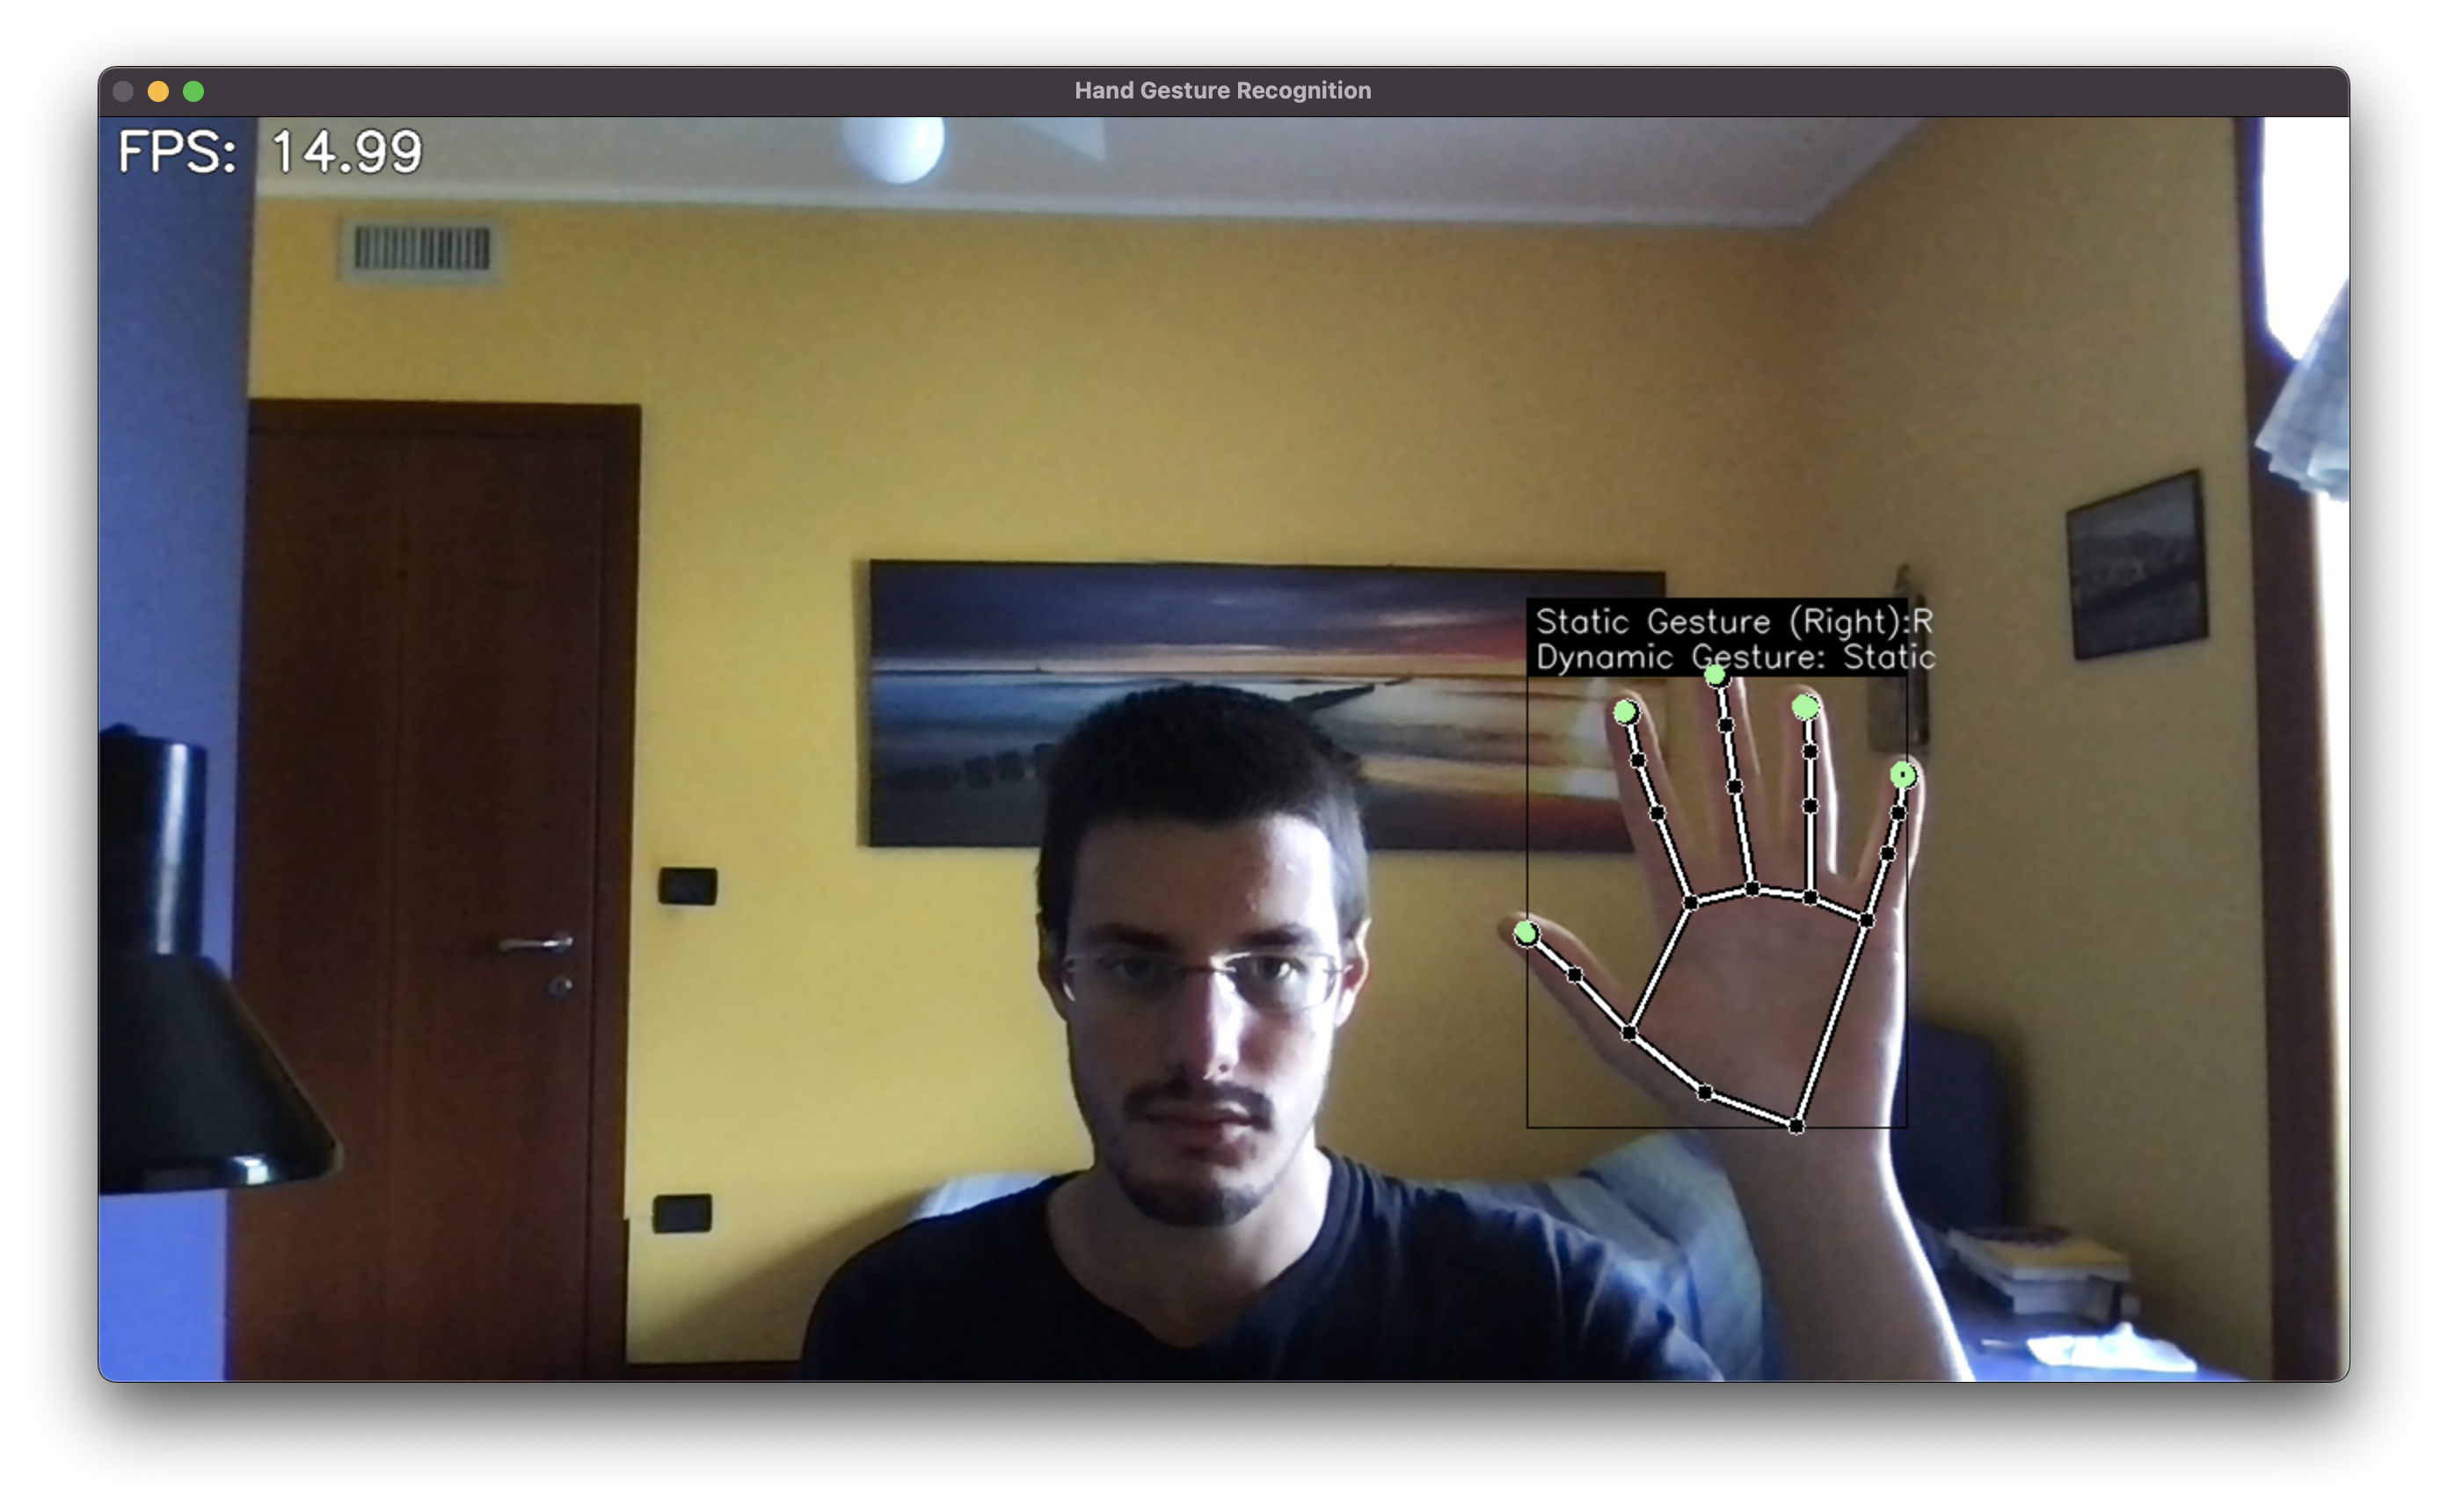
\includegraphics[width=\textwidth]{thesis/images/recognition_without_gloves.png}
        \caption{Hand tracking without glove.}
        \label{fig:ht_without_gloves}
    \end{subfigure}
    \hfill
    \begin{subfigure}[b]{1\textwidth}
        \centering
        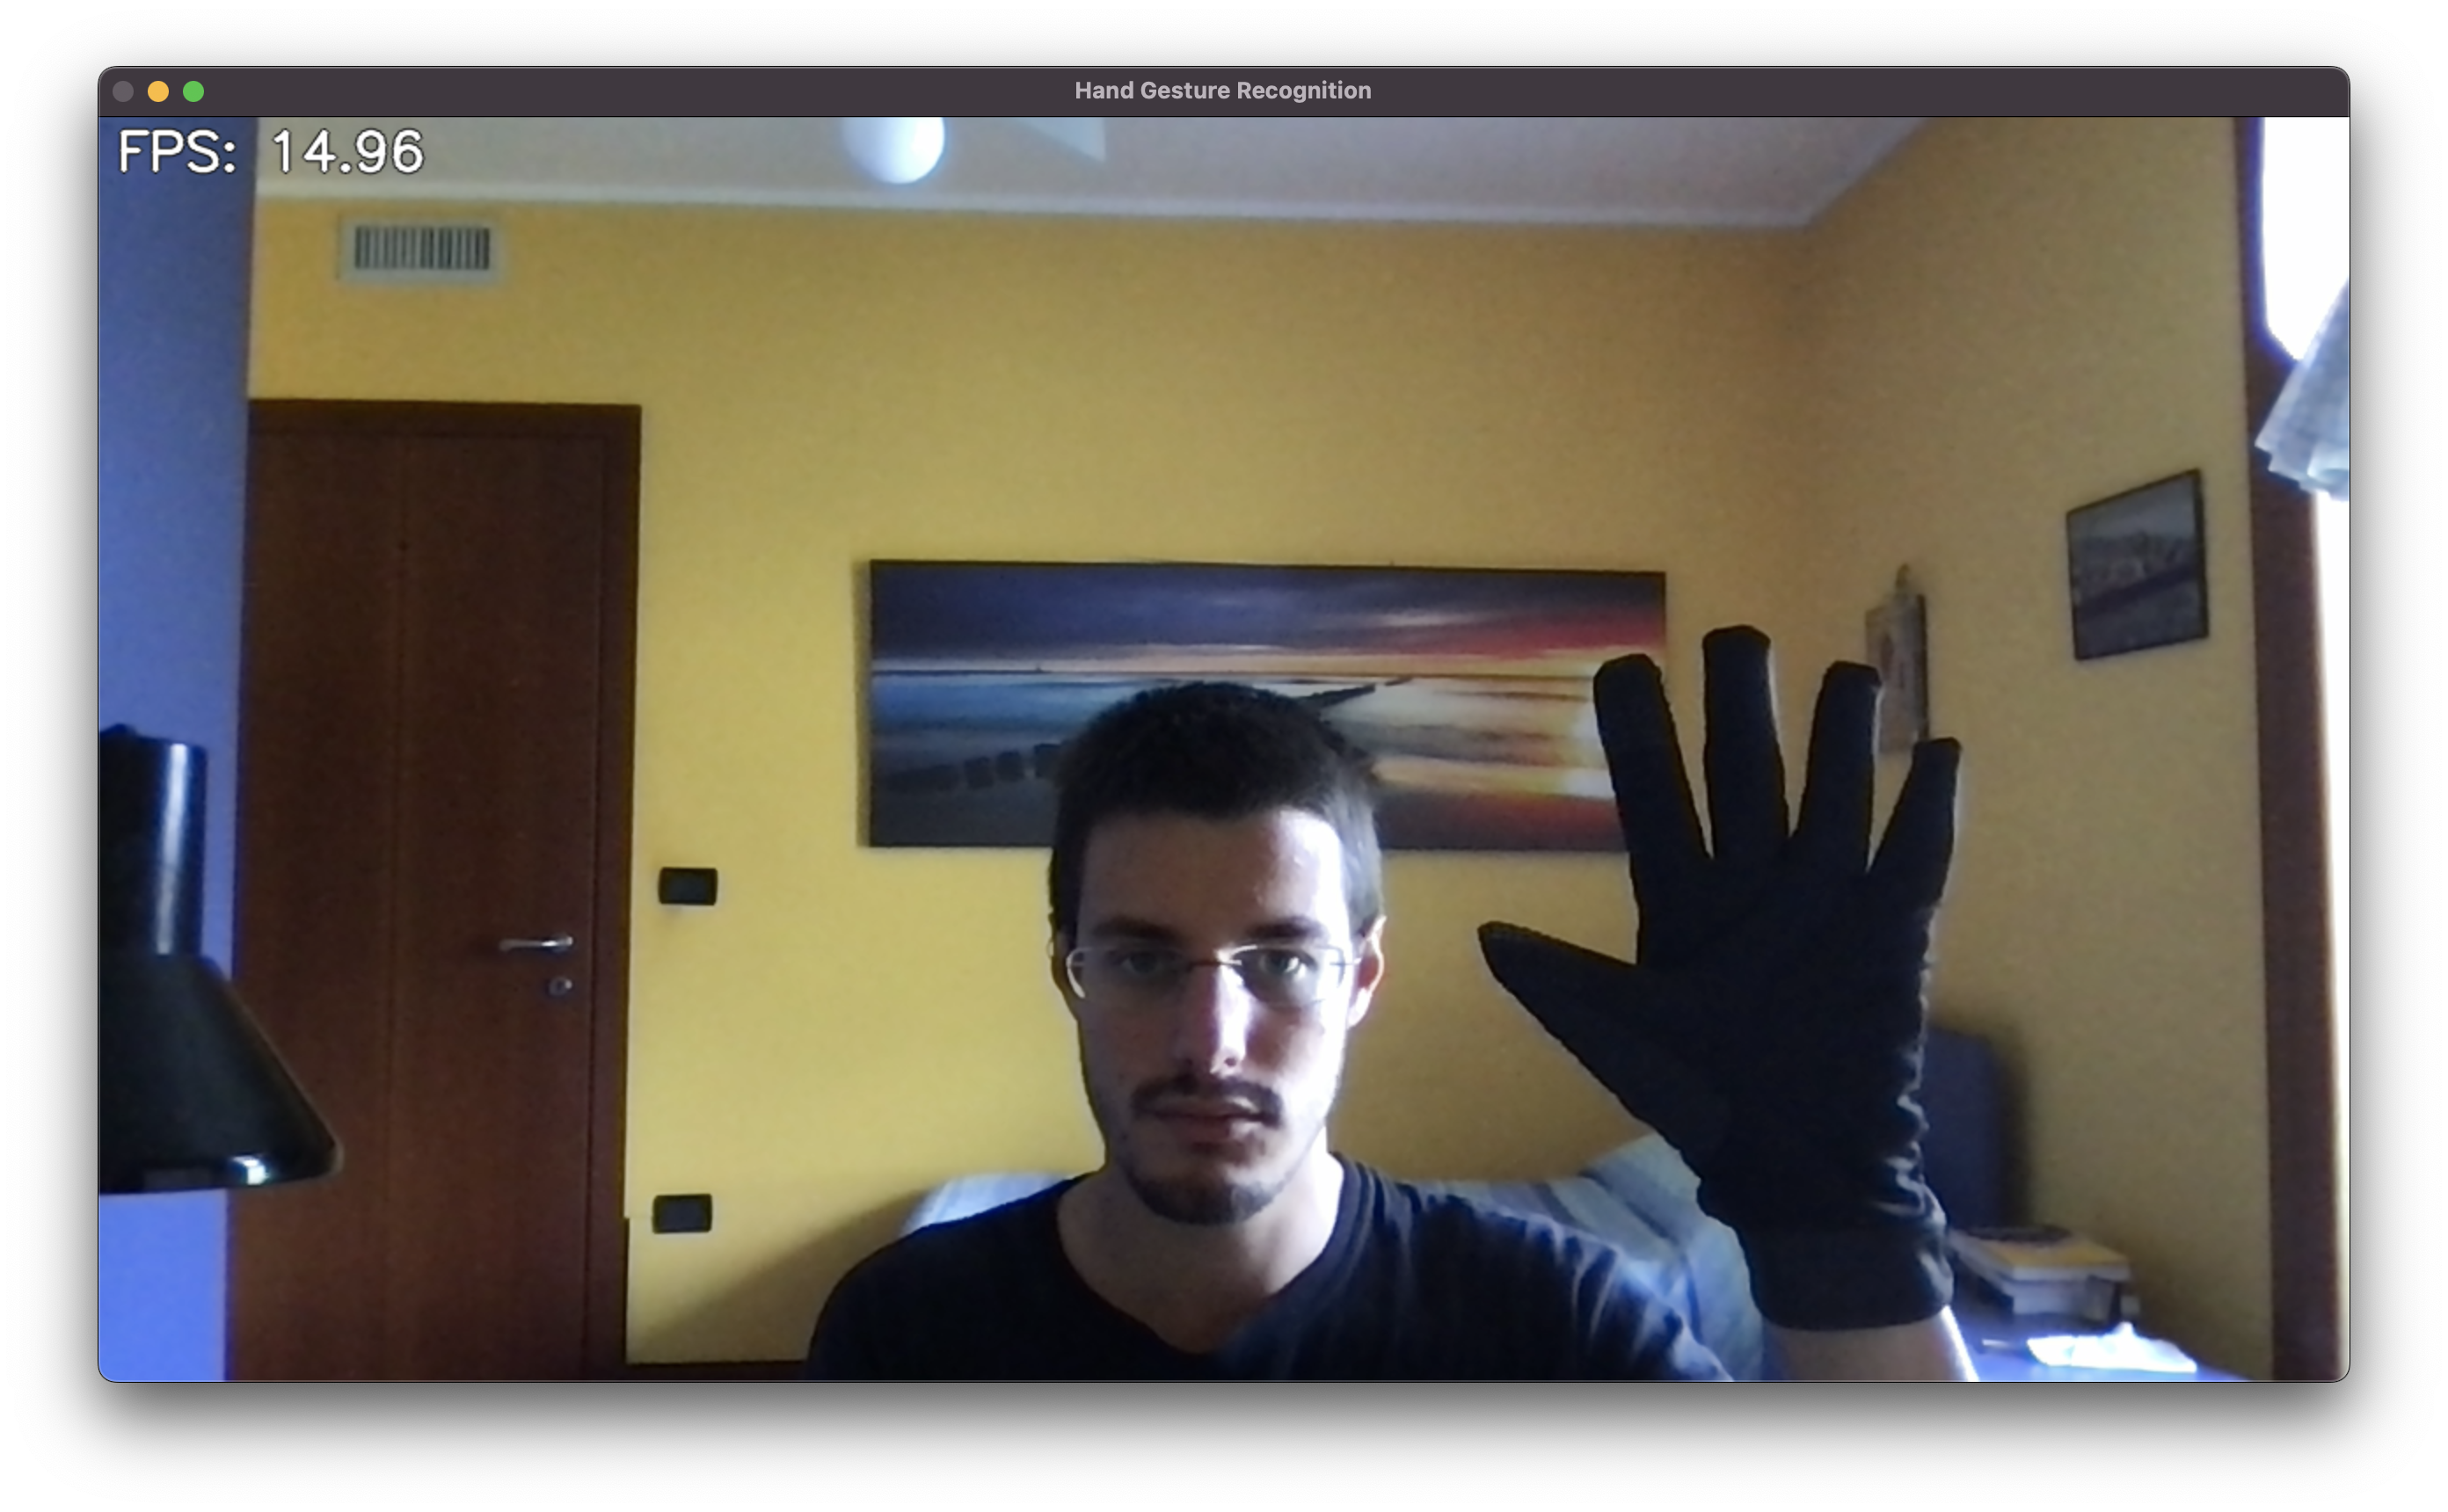
\includegraphics[width=\textwidth]{thesis/images/recognition_with_gloves.png}
        \caption{Hand tracking with glove.}
        \label{fig:ht_with_gloves}
    \end{subfigure}
    \caption{Difference between wearing a glove and not for MediaPipe.}
    \label{fig:ht_with_and_without_glove}
\end{figure}
\end{document}